\section{Implementation details}
\label{app:impl}

\paragraph{Model and checkpoints.} We use the official MDM code \citep{tevet2023mdm} and its HumanML3D encoder checkpoints with 50 and 1000 diffusion steps. Both have the same architecture and text encoder, but they were trained with different releases of the code, and their saved training settings differ beyond the number of steps (each checkpoint's \texttt{args.json}); we therefore treat them as two models, not as a controlled comparison of step counts. Joint positions are recovered from the 263-dimensional HumanML3D features with the dataset's normalization statistics; no SMPL body model is needed. Each layer's output is recorded with a forward hook after the condition token is dropped; in the main runs we keep every fourth frame (30 per motion), and the noisy input and the clean-motion estimate are stored at the same frames.

\paragraph{Compute.} All experiments ran on a single laptop GPU (Apple M4 Pro). A forward pass on the laptop GPU matches the CPU to about $10^{-4}$ relative error in every layer. Sampling 1,000 motions takes about 2 minutes with the 50-step model and under an hour with the 1000-step model. The SMPL bodies in the figures are fitted to the generated joints for display only, with mean joint errors of 1.0 to 3.0\,cm per figure (largest for two of the extreme jumps in Figure~\ref{fig:layerknows}c). All probes, controls and simulations run on cached arrays in minutes to an hour. Code that reproduces every experiment, table and figure, from sampling to the final plots, is available at \url{https://github.com/saeed1262/motion-physics-probing}.

\paragraph{Body meshes in Figure~\ref{fig:teaser}.} For display only, we fit the neutral SMPL body \citep{loper2015smpl} to the 22 joints of each drawn frame with the SMPLify-style fitter distributed with MDM \citep{bogo2016keep} (150 iterations). The mean distance between fitted and generated joints is 1.0 to 1.2\,cm across the six rows. The lowest mesh vertex lies 1.2 to 6.5\,cm below the lowest foot joint, as expected since the ankle and toe joints sit inside the foot, so a floating body's sole stays visibly above its shadow.

\paragraph{Prompts.} The 64 curated prompts (each preceded by ``a person'') are:
{\small walks forward; walks forward slowly and carefully; jogs forward; runs forward quickly; walks in a circle; walks backward; sidesteps to the left; walks forward and turns around; jumps up in place; jumps forward; does a long jump forward; hops on their left leg; hops on their right leg; jumps over an obstacle; skips forward; does jumping jacks; jumps up and spins in the air; leaps to the side; runs and jumps; jumps backward; jumps with both feet three times; jumps and lands on one foot; stands on one leg; balances on their right foot with arms out; leans forward; leans to the left; stands on their toes; walks on a balance beam; loses balance and catches themselves; stumbles forward; bends down to touch their toes; squats down and stands up; does a lunge forward; kicks with their right leg; kicks high with their left leg; does a yoga tree pose; tiptoes forward; runs and then stops suddenly; waves with their right hand; throws a ball; picks something up from the ground; reaches up high; claps their hands; stretches their arms; punches forward; boxes; swings a golf club; kicks a soccer ball; dances; does a spin; marches in place; crouches and walks; walks while carrying something heavy; dribbles a basketball and shoots; plays tennis; shuffles side to side; steps forward and back; turns in place; stands still; stretches their legs; shakes their body; runs in a zigzag; jogs in place; sprints.}

The 186 test captions are drawn at random (fixed seed) from the HumanML3D test split, one caption per motion, keeping captions of 3 to 20 words that do not duplicate a curated prompt.

\paragraph{Readouts.} Per-frame probes predict the final motion's label at the same frame. Ridge probes use standardized inputs and choose the penalty from $\{1, 10, 100, 1000, 10^4\}$ by efficient leave-one-out cross-validation. The \emph{Estimate, MLP} readout concatenates the estimate's 263 features with the dynamic and static balance margins, lowest-foot height, in-flight and airborne flags and foot sliding speed computed from the estimate (and, for the gravity target, its flight gravity), each with an indicator for undefined values (undefined values set to zero), and its four foot-contact flags. Where the estimate's own label is undefined, the explicit readout uses the median of its defined values. The MLP (two hidden layers of 256 units, ReLU, dropout 0.1) is trained on standardized inputs and targets with AdamW (learning rate $10^{-3}$, weight decay $10^{-4}$, batch 512) for up to 100 epochs, stopping after 8 epochs without improvement on 15\% of the training prompts, held out as a group; the same settings are used for every feature set. Fixed layers: dynamic and static balance, layer 7; flight, layer 6; flight gravity, layer 5.

\paragraph{Temporal readout.} To test whether per-frame readouts handicap the estimate on quantities that need several frames, a small temporal network reads all 30 recorded frames of a motion and predicts the final motion's label at every frame: two 1D convolutions over time (128 channels, kernel 5, the second dilated by 2, GELU, dropout 0.1) and a per-frame linear output, trained with AdamW (learning rate $10^{-3}$, weight decay $10^{-3}$, batch 32) on a loss masked to labelled frames, with early stopping (patience 15, up to 200 epochs) on 15\% of the training prompts. Inputs are everything the estimate shows, the same fixed layer, or both, at 20\% of denoising; folds and scores are those of the per-frame readouts, one seed at a time. Trained per seed, it reads dynamic balance better from the estimate than from the layer in all six runs (by 0.014 to 0.034 in $R^2$), and flight as well (by 0.001 to 0.010 in AUC). For the fall rate on the jump prompts it reaches $R^2 = 0.297 \pm 0.017$ from the estimate and $0.379 \pm 0.025$ from the layer on the 50-step model, and $0.290 \pm 0.114$ and $0.344 \pm 0.124$ on the 1000-step model, with the layer ahead in every seed (by 0.038 to 0.097).

\paragraph{Tuned readouts.} With seeds pooled, the five folds are grouped by prompt across seeds, and inside each outer fold 15\% of the training prompts form the validation split used for every choice. Ridge selects its penalty from $\{10^{-1}, 1, \dots, 10^{6}\}$ on that split (inputs standardized, targets centred) and is refit on all training frames. The MLP family is $f(x) = w^\top x + b + \mathrm{MLP}(x)$, so that it contains the linear readout, trained on standardized inputs and targets with AdamW (learning rate $10^{-3}$, batch 1024) for up to 80 epochs, stopping after 6 epochs without improvement on the validation split. Its five configurations are (hidden units, hidden layers, dropout, weight decay): $(256, 2, 0.1, 10^{-4})$, the fixed MLP's settings; $(256, 2, 0.3, 10^{-2})$; $(64, 2, 0.1, 10^{-3})$; $(1024, 1, 0.3, 10^{-2})$; and $(1024, 2, 0.3, 10^{-3})$. The configuration and the family with the lowest validation error are kept, separately in each outer fold. Ridge is then refit on all training frames, while the MLP keeps the fit on the 85\% used with early stopping. Selection uses mean squared error for every target, including flight and floats or falls, which are scored by AUC. The MLP family was selected in 70 to 100\% of folds per data set, and every configuration at least once. The same fixed layers are used as above for MDM, and Section~\ref{sec:models} gives MotionDiffuse's. The readout of estimate and layer with fallback chooses among the 12 candidates of both input sets (two ridge fits and ten MLPs over the two inputs, counting the estimate's) by the same validation error. Over MDM's four data sets it picks the estimate alone in 25 of the 40 folds for balance and flight, and in 1 of the 10 for the fall rate on the jump prompts. Our per-frame inputs omit the condition token (token 0 of the encoder). To test it, we recorded the 50-step model's three main runs again with the token kept (the motions, and the estimate's scores, are identical); adding the token's output at the same layer (the same for every frame of a motion) to the readout of estimate and layer gains $-0.001$ [$-0.003$, $0.002$] for dynamic balance, $+0.004$ [$-0.000$, $0.009$] for flight and $+0.002$ [$-0.003$, $0.007$] for whether a body floats or falls (tuned with fallback; with all eight layers, $0.000$, $0.000$ and $-0.007$). Table~\ref{tab:raw} separates the two ways in which the estimate's readout differs from the layer's: the input (the estimate's 263 raw features, or everything it shows) and the family. With raw features the tuned estimate ties the tuned layer for balance and flight on MDM; the labels computed from the estimate, which are fixed functions of it, add about 0.02 in $R^2$ for dynamic balance.

\begin{table}[h]
\centering
\caption{Pooled scores at 20\% of denoising, seeds pooled: the estimate read from its raw features or from everything it shows, and the layer, each with ridge and with the tuned MLP family. $^\dagger$The MLP family diverged in one fold, in every configuration (MotionDiffuse, fall rate, inputs that include the estimate's labels); the tuned readouts chose ridge in that fold, so Table~\ref{tab:tuned} is unaffected.}
\label{tab:raw}
\resizebox{\linewidth}{!}{\begin{tabular}{llcccccc}
\toprule
& & \multicolumn{4}{c}{Estimate} & \multicolumn{2}{c}{Layer} \\
\cmidrule(lr){3-6} \cmidrule(lr){7-8}
Target & Model & raw, ridge & raw, MLP & all it shows, ridge & all it shows, MLP & ridge & MLP \\
\midrule
Dynamic balance & 50-step & 0.767 & 0.869 & 0.866 & 0.889 & 0.850 & 0.862 \\
Dynamic balance & 1000-step & 0.594 & 0.762 & 0.746 & 0.779 & 0.720 & 0.765 \\
Dynamic balance & MotionDiffuse & 0.583 & 0.825 & 0.606 & 0.823 & 0.620 & 0.700 \\
Static balance & 50-step & 0.697 & 0.798 & 0.825 & 0.830 & 0.780 & 0.801 \\
Static balance & 1000-step & 0.544 & 0.646 & 0.641 & 0.671 & 0.592 & 0.647 \\
Static balance & MotionDiffuse & 0.511 & 0.726 & 0.536 & 0.729 & 0.537 & 0.568 \\
In flight & 50-step & 0.944 & 0.975 & 0.974 & 0.976 & 0.977 & 0.971 \\
In flight & 1000-step & 0.903 & 0.933 & 0.919 & 0.935 & 0.934 & 0.932 \\
In flight & MotionDiffuse & 0.963 & 0.944 & 0.967 & 0.943 & 0.951 & 0.898 \\
In flight & 50-step, jump prompts & 0.971 & 0.982 & 0.979 & 0.984 & 0.981 & 0.981 \\
In flight & 1000-step, jump prompts & 0.940 & 0.960 & 0.949 & 0.960 & 0.955 & 0.961 \\
In flight & MotionDiffuse, jump prompts & 0.977 & 0.977 & 0.977 & 0.975 & 0.978 & 0.972 \\
Floats or falls & 50-step & 0.976 & 0.979 & 0.982 & 0.980 & 0.990 & 0.989 \\
Floats or falls & 1000-step & 0.949 & 0.958 & 0.963 & 0.964 & 0.980 & 0.976 \\
Floats or falls & MotionDiffuse & 0.932 & 0.947 & 0.941 & 0.935 & 0.988 & 0.975 \\
Floats or falls & 50-step, jump prompts & 0.952 & 0.962 & 0.978 & 0.974 & 0.971 & 0.969 \\
Floats or falls & 1000-step, jump prompts & 0.958 & 0.963 & 0.962 & 0.966 & 0.973 & 0.969 \\
Floats or falls & MotionDiffuse, jump prompts & 0.833 & 0.781 & 0.841 & 0.826 & 0.836 & 0.788 \\
Fall rate (falling only) & 50-step & $-0.096$ & $-0.372$ & $-0.051$ & 0.031 & 0.267 & 0.217 \\
Fall rate (falling only) & 1000-step & $-0.097$ & $-0.040$ & $-0.055$ & $-0.008$ & 0.115 & 0.054 \\
Fall rate (falling only) & 50-step, jump prompts & 0.183 & 0.267 & 0.273 & 0.351 & 0.374 & 0.427 \\
Fall rate (falling only) & 1000-step, jump prompts & 0.035 & 0.195 & 0.206 & 0.287 & 0.273 & 0.309 \\
Fall rate (falling only) & MotionDiffuse, jump prompts & 0.213 & 0.239 & 0.370 & $-59.7^\dagger$ & 0.326 & 0.231 \\
\bottomrule
\end{tabular}
}
\end{table}

\begin{table}[h]
\centering
\caption{The gain from adding the layer in detail (20\% of denoising, seeds pooled, pooled score, 95\% prompt-bootstrap intervals). With fallback: as in Table~\ref{tab:tuned}. Without fallback: the tuned readout of estimate and layer against the tuned estimate. Estimate kept: outer folds, of five, in which the fallback chose a readout of the estimate alone, so that fold's gain is zero by construction; when all five do, no interval is defined. Rescaled: for $R^2$, the conditional usable information in nats by Proposition~\ref{prop:vinfo}, $\tfrac12 \log\big((1 - R^2_{\text{estimate}})/(1 - R^2_{\text{both}})\big)$; for AUC, the share of misranked pairs that adding the layer removes.}
\label{tab:gaindetail}
\resizebox{\linewidth}{!}{\begin{tabular}{llcccc}
\toprule
Target & Model & Gain with fallback & Gain without fallback & Estimate kept & Gain, rescaled \\
\midrule
Dynamic balance & 50-step & $+0.000$ [$-0.001$, $+0.001$] & $-0.005$ [$-0.010$, $-0.000$] & 4 & +0.001 \\
Dynamic balance & 1000-step & $-0.002$ [$-0.005$, $-0.000$] & $-0.002$ [$-0.006$, $+0.002$] & 3 & $-$0.006 \\
Dynamic balance & MotionDiffuse & $0$ (all folds) & $-0.015$ [$-0.023$, $-0.007$] & 5 & +0.000 \\
\addlinespace[2pt]
Static balance & 50-step & $-0.001$ [$-0.004$, $+0.002$] & $-0.004$ [$-0.008$, $-0.000$] & 2 & $-$0.004 \\
Static balance & 1000-step & $0$ (all folds) & $-0.006$ [$-0.018$, $+0.002$] & 5 & +0.000 \\
Static balance & MotionDiffuse & $0$ (all folds) & $-0.031$ [$-0.051$, $-0.012$] & 5 & +0.000 \\
\addlinespace[2pt]
In flight & 50-step & $-0.004$ [$-0.008$, $-0.000$] & $-0.004$ [$-0.009$, $+0.002$] & 2 & $-$15\% \\
In flight & 1000-step & $-0.000$ [$-0.003$, $+0.002$] & $+0.003$ [$-0.003$, $+0.009$] & 4 & $-$1\% \\
In flight & MotionDiffuse & $-0.004$ [$-0.009$, $-0.001$] & $-0.006$ [$-0.026$, $+0.018$] & 4 & $-$8\% \\
In flight & 50-step, jump prompts & $-0.001$ [$-0.002$, $-0.000$] & $-0.002$ [$-0.004$, $-0.001$] & 4 & $-$5\% \\
In flight & 1000-step, jump prompts & $+0.001$ [$-0.000$, $+0.003$] & $+0.002$ [$+0.000$, $+0.005$] & 1 & +4\% \\
In flight & MotionDiffuse, jump prompts & $+0.000$ [$-0.001$, $+0.002$] & $-0.003$ [$-0.006$, $-0.000$] & 4 & +1\% \\
\addlinespace[2pt]
Floats or falls & 50-step & $+0.008$ [$+0.001$, $+0.015$] & $+0.011$ [$+0.003$, $+0.021$] & 1 & +39\% \\
Floats or falls & 1000-step & $+0.003$ [$-0.001$, $+0.008$] & $+0.011$ [$+0.005$, $+0.019$] & 2 & +10\% \\
Floats or falls & MotionDiffuse & $+0.026$ [$+0.007$, $+0.055$] & $+0.033$ [$+0.012$, $+0.064$] & 2 & +43\% \\
Floats or falls & 50-step, jump prompts & $-0.000$ [$-0.009$, $+0.008$] & $+0.001$ [$-0.009$, $+0.009$] & 2 & $-$0\% \\
Floats or falls & 1000-step, jump prompts & $+0.001$ [$-0.001$, $+0.003$] & $+0.003$ [$+0.000$, $+0.006$] & 1 & +3\% \\
Floats or falls & MotionDiffuse, jump prompts & $+0.001$ [$-0.017$, $+0.017$] & $+0.022$ [$-0.003$, $+0.054$] & 2 & +0\% \\
\addlinespace[2pt]
Fall rate (falling only) & 50-step & $+0.253$ [$+0.060$, $+0.505$] & $+0.408$ [$+0.178$, $+0.642$] & 2 & +0.122 \\
Fall rate (falling only) & 1000-step & $+0.082$ [$-0.035$, $+0.167$] & $+0.231$ [$+0.079$, $+0.409$] & 1 & +0.040 \\
Fall rate (falling only) & 50-step, jump prompts & $+0.077$ [$+0.051$, $+0.107$] & $+0.077$ [$+0.051$, $+0.107$] & 0 & +0.063 \\
Fall rate (falling only) & 1000-step, jump prompts & $+0.076$ [$+0.053$, $+0.096$] & $+0.082$ [$+0.060$, $+0.102$] & 1 & +0.056 \\
Fall rate (falling only) & MotionDiffuse, jump prompts & $+0.025$ [$+0.003$, $+0.047$] & $+0.034$ [$+0.009$, $+0.060$] & 2 & +0.020 \\
\bottomrule
\end{tabular}
}
\end{table}

\begin{table}[h]
\centering
\caption{Noise level at the recorded steps: $\bar\alpha_t$ and the signal-to-noise ratio $\bar\alpha_t / (1 - \bar\alpha_t)$ of the noisy input, from each model's schedule (MDM cosine, MotionDiffuse linear; \texttt{scripts/noise\_levels.py}).}
\label{tab:snr}
\begin{tabular}{lcccccccc}
\toprule
& \multicolumn{2}{c}{20\%} & \multicolumn{2}{c}{40\%} & \multicolumn{2}{c}{60\%} & \multicolumn{2}{c}{80\%} \\
\cmidrule(lr){2-3} \cmidrule(lr){4-5} \cmidrule(lr){6-7} \cmidrule(lr){8-9}
Model & $\bar\alpha$ & SNR & $\bar\alpha$ & SNR & $\bar\alpha$ & SNR & $\bar\alpha$ & SNR \\
\midrule
MDM, 50-step & 0.094 & 0.104 & 0.341 & 0.517 & 0.617 & 1.614 & 0.879 & 7.273 \\
MDM, 1000-step & 0.094 & 0.104 & 0.341 & 0.517 & 0.646 & 1.825 & 0.898 & 8.781 \\
MotionDiffuse & 0.002 & 0.002 & 0.026 & 0.027 & 0.194 & 0.240 & 0.656 & 1.910 \\
\bottomrule
\end{tabular}

\end{table}

\begin{table}[h]
\centering
\caption{Positive control (50-step model, 20\% of denoising, seeds pooled; gain with fallback over the tuned estimate, 95\% prompt-bootstrap intervals). Injected: the tuned estimate readout's out-of-fold residual plus noise, sized so that its best linear use would add the stated $R^2$ on the squared-error scale, added to the layer along one random direction with the variance of a typical direction of the standardized activations (\texttt{fair\_readouts.py -{}-layer-spec inject}). Tuned readouts can extract more than this linear amount. The real-layer rows come from the same rerun as the injected rows and differ from Table~\ref{tab:tuned} by refit noise of at most 0.001.}
\label{tab:control}
\resizebox{\linewidth}{!}{\begin{tabular}{llcc}
\toprule
& Added to the estimate & Pooled score & Within prompt and frame \\
\midrule
Dynamic balance ($R^2$) & the layer (real) & $+0.000$ [$-0.001$, $+0.001$] & $+0.000$ [$-0.001$, $+0.001$] \\
 & injected, 0.005 & $+0.013$ [$+0.009$, $+0.017$] & $+0.018$ [$+0.013$, $+0.022$] \\
 & injected, 0.01 & $+0.025$ [$+0.020$, $+0.030$] & $+0.035$ [$+0.031$, $+0.040$] \\
 & injected, 0.02 & $+0.040$ [$+0.034$, $+0.047$] & $+0.055$ [$+0.049$, $+0.061$] \\
\addlinespace[2pt]
In flight (AUC) & the layer (real) & $-0.004$ [$-0.008$, $+0.000$] & $-0.008$ [$-0.014$, $-0.002$] \\
 & injected, 0.005 & $-0.010$ [$-0.021$, $-0.002$] & $+0.018$ [$+0.009$, $+0.028$] \\
 & injected, 0.01 & $+0.001$ [$-0.006$, $+0.008$] & $+0.042$ [$+0.030$, $+0.056$] \\
 & injected, 0.02 & $+0.001$ [$-0.006$, $+0.008$] & $+0.072$ [$+0.057$, $+0.092$] \\
\addlinespace[2pt]
Floats or falls, jump prompts (AUC) & the layer (real) & $-0.000$ [$-0.008$, $+0.008$] & $-0.000$ [$-0.014$, $+0.016$] \\
 & injected, 0.005 & $+0.001$ [$-0.005$, $+0.007$] & $+0.006$ [$-0.014$, $+0.024$] \\
 & injected, 0.01 & $+0.002$ [$-0.008$, $+0.011$] & $+0.030$ [$+0.002$, $+0.059$] \\
 & injected, 0.02 & $+0.004$ [$-0.005$, $+0.012$] & $+0.057$ [$+0.030$, $+0.085$] \\
\bottomrule
\end{tabular}
}
\end{table}

\paragraph{Sample-level prediction.} Per-sample failure rates are predicted from frame-averaged activations with ridge regression ($\alpha = 10$; $\alpha = 100$ for the CLIP text embedding) in prompt-grouped 5-fold cross-validation. The layer used for the within-prompt comparison is chosen on the first seed by its mean within-prompt correlation and then evaluated on the other seeds.

\paragraph{Early-warning simulation.} For each prompt we pool its recorded samples across seeds and simulate 200 requests. A request draws a sample uniformly with replacement; an aborted attempt costs $k+1$ steps for a check at step $k$, a completed one costs the full number of steps; the last allowed attempt is always delivered. Compute at matched failure is interpolated along each strategy's curve over retry budgets 1 to 20, at the failure rates that finish-then-filter reaches with 2, 3 and 5 tries; larger budgets reach a floor set by prompts that float in nearly every sample.

\section{The fair comparison with a fixed MLP, per seed, and the pilot}
\label{app:fixedmlp}

\begin{figure}[h]
\centering
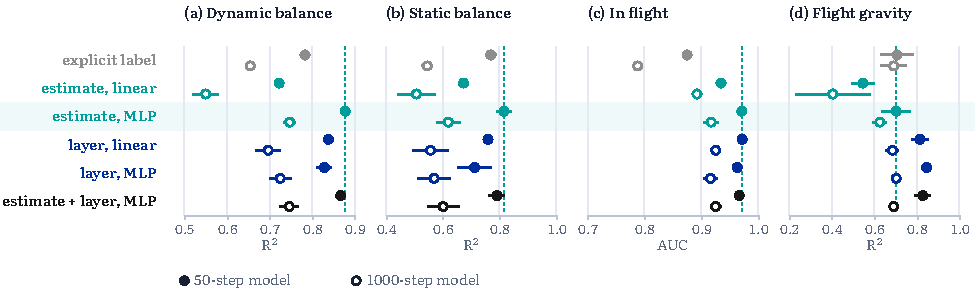
\includegraphics[width=\linewidth]{figures/web/fig_fair.pdf}
\caption{Fair comparison at 20\% of denoising. Each row is a readout; filled circles show the 50-step model and open circles the 1000-step model (mean, with the standard deviation over seeds). The dashed line marks the MLP on everything the estimate shows (shaded row) for the 50-step model. For both balance measures it matches or beats every readout that uses the layer on both MDM checkpoints, and adding the layer to it (black) does not help; for flight this holds on the 50-step model, while on the 1000-step model the layer's linear probe is slightly ahead (0.926 against 0.918). Flight gravity is the exception in these data, on both checkpoints; Section~\ref{sec:fairresults} tests it with tuned readouts and about ten times as many falling frames.}
\label{fig:fair}
\end{figure}

\begin{table}[h]
\centering
\caption{Pooled scores at 20\% of denoising (mean $\pm$ standard deviation over seeds; best per row in bold). Estimate, MLP reads everything the estimate shows; Estimate + layer adds the layer's activations.}
\label{tab:fair}
\resizebox{\linewidth}{!}{%
\begin{tabular}{llcccccc}
\toprule
Model & Target & Explicit & Estimate, linear & Estimate, MLP & Layer, linear & Layer, MLP & Estimate + layer, MLP \\
\midrule
\multirow{4}{*}{50-step} & Dynamic balance ($R^2$) & 0.783 $\pm$ 0.009 & 0.723 $\pm$ 0.007 & \textbf{0.878 $\pm$ 0.005} & 0.838 $\pm$ 0.001 & 0.829 $\pm$ 0.018 & 0.867 $\pm$ 0.007 \\
 & Static balance ($R^2$) & 0.769 $\pm$ 0.019 & 0.673 $\pm$ 0.014 & \textbf{0.816 $\pm$ 0.028} & 0.759 $\pm$ 0.014 & 0.712 $\pm$ 0.059 & 0.791 $\pm$ 0.028 \\
 & In flight (AUC) & 0.876 $\pm$ 0.005 & 0.935 $\pm$ 0.008 & 0.972 $\pm$ 0.001 & \textbf{0.972 $\pm$ 0.003} & 0.964 $\pm$ 0.004 & 0.967 $\pm$ 0.008 \\
 & Flight gravity ($R^2$) & 0.707 $\pm$ 0.079 & 0.547 $\pm$ 0.053 & 0.703 $\pm$ 0.068 & 0.814 $\pm$ 0.040 & \textbf{0.846 $\pm$ 0.010} & 0.828 $\pm$ 0.038 \\
\midrule
\multirow{4}{*}{1000-step} & Dynamic balance ($R^2$) & 0.655 $\pm$ 0.008 & 0.550 $\pm$ 0.031 & \textbf{0.747 $\pm$ 0.014} & 0.697 $\pm$ 0.029 & 0.725 $\pm$ 0.026 & 0.746 $\pm$ 0.022 \\
 & Static balance ($R^2$) & 0.546 $\pm$ 0.019 & 0.508 $\pm$ 0.066 & \textbf{0.620 $\pm$ 0.043} & 0.557 $\pm$ 0.063 & 0.570 $\pm$ 0.058 & 0.601 $\pm$ 0.057 \\
 & In flight (AUC) & 0.788 $\pm$ 0.003 & 0.893 $\pm$ 0.001 & 0.918 $\pm$ 0.013 & \textbf{0.926 $\pm$ 0.002} & 0.917 $\pm$ 0.013 & 0.926 $\pm$ 0.010 \\
 & Flight gravity ($R^2$) & 0.691 $\pm$ 0.060 & 0.405 $\pm$ 0.176 & 0.627 $\pm$ 0.033 & 0.686 $\pm$ 0.030 & \textbf{0.703 $\pm$ 0.016} & 0.691 $\pm$ 0.013 \\
\bottomrule
\end{tabular}}

\end{table}

\begin{table}[h]
\centering
\caption{Within-prompt scores at 20\% of denoising: Pearson $r$ after subtracting each prompt's mean from target and prediction, so that only sample-specific information counts (mean $\pm$ standard deviation over seeds; best per row in bold).}
\label{tab:fairwithin}
\resizebox{\linewidth}{!}{%
\begin{tabular}{llcccccc}
\toprule
Model & Target & Explicit & Estimate, linear & Estimate, MLP & Layer, linear & Layer, MLP & Estimate + layer, MLP \\
\midrule
\multirow{4}{*}{50-step} & Dynamic balance ($r$) & 0.797 $\pm$ 0.011 & 0.756 $\pm$ 0.007 & \textbf{0.892 $\pm$ 0.003} & 0.851 $\pm$ 0.000 & 0.867 $\pm$ 0.002 & 0.889 $\pm$ 0.002 \\
 & Static balance ($r$) & 0.746 $\pm$ 0.020 & 0.644 $\pm$ 0.025 & \textbf{0.801 $\pm$ 0.023} & 0.729 $\pm$ 0.015 & 0.749 $\pm$ 0.020 & 0.795 $\pm$ 0.019 \\
 & In flight ($r$) & 0.710 $\pm$ 0.007 & 0.562 $\pm$ 0.014 & 0.755 $\pm$ 0.010 & 0.662 $\pm$ 0.010 & 0.734 $\pm$ 0.007 & \textbf{0.760 $\pm$ 0.008} \\
 & Flight gravity ($r$) & 0.439 $\pm$ 0.053 & 0.219 $\pm$ 0.047 & 0.340 $\pm$ 0.039 & 0.445 $\pm$ 0.071 & \textbf{0.536 $\pm$ 0.109} & 0.508 $\pm$ 0.081 \\
\midrule
\multirow{4}{*}{1000-step} & Dynamic balance ($r$) & 0.736 $\pm$ 0.004 & 0.664 $\pm$ 0.008 & 0.816 $\pm$ 0.001 & 0.772 $\pm$ 0.011 & 0.800 $\pm$ 0.006 & \textbf{0.817 $\pm$ 0.003} \\
 & Static balance ($r$) & 0.607 $\pm$ 0.010 & 0.572 $\pm$ 0.010 & \textbf{0.679 $\pm$ 0.003} & 0.610 $\pm$ 0.010 & 0.642 $\pm$ 0.010 & 0.673 $\pm$ 0.005 \\
 & In flight ($r$) & 0.562 $\pm$ 0.012 & 0.502 $\pm$ 0.020 & 0.608 $\pm$ 0.035 & 0.556 $\pm$ 0.024 & 0.580 $\pm$ 0.025 & \textbf{0.612 $\pm$ 0.034} \\
 & Flight gravity ($r$) & \textbf{0.645 $\pm$ 0.079} & 0.405 $\pm$ 0.101 & 0.576 $\pm$ 0.020 & 0.572 $\pm$ 0.023 & 0.614 $\pm$ 0.012 & 0.616 $\pm$ 0.003 \\
\bottomrule
\end{tabular}}

\end{table}

The first version of the fair comparison uses one fixed MLP (Section~\ref{sec:fair}) per seed. Figure~\ref{fig:fair} and Tables~\ref{tab:fair} and \ref{tab:fairwithin} replace the explicit label and the linear probe on the estimate with the same MLP that reads the layer. For both balance measures, the MLP on the estimate beats both the layer's linear probe and the same MLP on the layer, on both checkpoints; for dynamic balance on the 50-step model it scores 0.878, against 0.838 and 0.829. Adding the layer to the estimate changes $R^2$ by $-0.018$ to $-0.007$ for dynamic balance and by $-0.026$ to $-0.023$ for static balance on the 50-step model, and by $-0.012$ to $+0.005$ and $-0.037$ to $-0.002$ on the 1000-step model. For flight the readouts tie at an AUC of 0.97 on the 50-step model, and adding the layer changes the AUC by $-0.012$ to $+0.012$ across both MDM checkpoints. Within prompts (Table~\ref{tab:fairwithin}) the ordering is the same, so the conclusion does not rest on differences between prompts.

\begin{figure}[h]
\centering
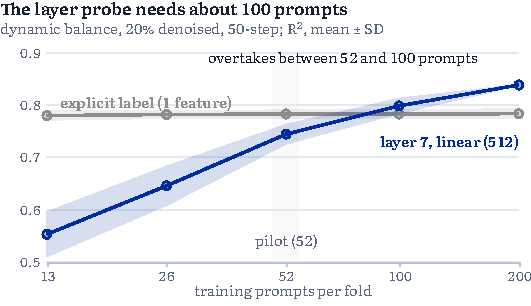
\includegraphics[width=0.55\linewidth]{figures/web/fig_learning.pdf}
\caption{Dynamic balance at 20\% of denoising (50-step model) with the probes trained on fewer prompts; same test folds; each point averages three draws of the training prompts in each of the three seeds (lines: mean; bands: standard deviation). The 512-feature layer probe overtakes the one-feature explicit label between 52 and 100 training prompts; the pilot (gray band) trained on 52.}
\label{fig:learning}
\end{figure}

Figure~\ref{fig:learning} shows why the pilot of Section~\ref{sec:learning} pointed the other way, with the linear layer probe of Section~\ref{sec:readable} trained on fewer prompts. The explicit label has a single feature and barely depends on training size (mean $R^2$ 0.780 to 0.783 across sizes). The linear layer probe has 512 features and improves steadily, from 0.553 with 13 training prompts and 0.744 with 52 to 0.798 with 100 and 0.837 to 0.839 with all of them. Applied to the larger data, the pilot's exact split gives gaps of $-0.003$, $+0.022$ and $+0.049$ across seeds, so its 12-prompt test set was also too small to fix the sign. Whether the layers appear to know more or less than the model shows can thus be set by the amount of training data, independently of what the model represents.

\section{The airborne label and the floating stretches}
\label{app:labelfix}

Our first airborne rule required only that every foot joint be above its contact height. On one 50-step run (1,000 motions) this gave 418 airborne stretches of at least 0.2\,s: 209 ballistic ($\hat g > 5\,\mathrm{m/s^2}$, 163 from the curated jump prompts) and 195 with $|\hat g| < 2\,\mathrm{m/s^2}$, 191 of them from other prompts. Inspecting the latter:

\begin{center}
\begin{tabular}{lr}
\toprule
Near-zero-gravity stretch & Stretches \\
\midrule
Supported by another body part (a wrist or knee within 15\,cm of the floor) & 48 \\
Feet raised but nearly still (for example a balance beam) & 48 \\
Whole motion above the floor & 5 \\
Unsupported and not falling & 94 \\
\bottomrule
\end{tabular}
\end{center}

The unsupported cases are ordinary walking poses with the whole body 7 to 12\,cm off the floor (median lowest foot 8.3\,cm, median duration 0.6\,s) in motions whose lowest foot elsewhere is at the floor (median 2.0\,cm): a real floating artifact. A foot-clearance threshold does not separate the groups: requiring the lowest foot to rise above 15\,cm keeps 73\% of ballistic stretches but also 44\% of near-zero ones, because cartwheels and crawling lift the feet. We therefore exclude stretches supported by a knee, wrist or the pelvis, and split the remaining unsupported stretches by whether they fall (Section~\ref{sec:labels}). Raised feet with no other support still count as airborne; a scene-free label cannot tell a balance beam from floating. All results in the main text use the fixed label. Only gravity-related labels changed; readouts that take the estimate's airborne flag as an input moved by at most 0.013.

\section{Sensitivity to the label thresholds}
\label{app:sensitivity}

\begin{table}[h]
\centering
\caption{Label thresholds changed one at a time (range over the three seeds of each model; the early rule ``abort if the decoded estimate shows floating'' is scored over the seeds of both MDM checkpoints).}
\label{tab:sensitivity}
\resizebox{\linewidth}{!}{\begin{tabular}{lcccccc}
\toprule
& \multicolumn{2}{c}{Floating, test captions (\% of frames)} & \multicolumn{2}{c}{Jump gravity, curated jump prompts (m/s$^2$)} & \multicolumn{2}{c}{Early rule at 20\%} \\
\cmidrule(lr){2-3} \cmidrule(lr){4-5} \cmidrule(lr){6-7}
Setting & 50-step & 1000-step & 50-step & 1000-step & Precision & Recall \\
\midrule
Default & 3.8--4.7 & 8.6--9.7 & 9.54--9.75 & 9.13--9.22 & 0.73--0.89 & 0.44--0.68 \\
Contact heights $\times 0.75$ & 6.4--7.6 & 13.1--13.8 & 9.68--9.92 & 9.03--9.40 & 0.66--0.78 & 0.46--0.58 \\
Contact heights $\times 1.25$ & 2.8--3.6 & 6.1--6.6 & 9.39--9.72 & 9.18--9.38 & 0.77--0.94 & 0.49--0.69 \\
Support rule 10\,cm & 3.8--4.7 & 8.7--9.7 & 9.54--9.75 & 9.13--9.22 & 0.72--0.91 & 0.45--0.65 \\
Support rule 20\,cm & 3.8--4.7 & 8.6--9.6 & 9.54--9.75 & 9.13--9.22 & 0.74--0.90 & 0.44--0.67 \\
Floating cut-off 1\,m/s$^2$ & 3.7--4.6 & 8.5--9.5 & 9.54--9.66 & 9.03--9.22 & 0.77--0.89 & 0.45--0.69 \\
Floating cut-off 3\,m/s$^2$ & 3.9--4.7 & 8.7--9.8 & 9.54--9.75 & 9.18--9.36 & 0.77--0.89 & 0.46--0.68 \\
\bottomrule
\end{tabular}
}
\end{table}

We recomputed every label from the cached joints with one threshold changed at a time: the ankle and toe contact heights scaled by 0.75 and 1.25, the support rule at 10 and 20\,cm instead of 15\,cm, and the floating cut-off at 1 and 3\,m/s$^2$ instead of 2\,m/s$^2$ (Table~\ref{tab:sensitivity}). Contact heights move the floating rates the most, since they decide which low poses count as unsupported; the support rule and the cut-off barely matter. Under every setting, every 1000-step seed floats more than every 50-step seed on test captions, by a factor of 1.9 to 2.1 in the means, and the median gravity of jumps on curated jump prompts stays between 9.03 and 9.92\,m/s$^2$. The training-free early rule keeps a precision of 0.66 to 0.94 and a recall of 0.44 to 0.69 across settings, seeds and models.

We also reran the fixed-MLP comparison of Appendix~\ref{app:fixedmlp} at 20\% of denoising under each setting, on the first seed of each model (dynamic balance only under the contact settings, since it depends on no other threshold). Its conclusions do not change. For dynamic balance, the MLP on the estimate beats the layer's linear probe by 0.020 to 0.059 in $R^2$, and adding the layer to it changes $R^2$ by $-0.018$ to $+0.004$, while the standard comparison favors the layer over the explicit label by 0.031 to 0.102. For flight gravity (layer 5), adding the layer gains 0.023 to 0.102, as with the default thresholds. The floating cut-off does not enter the probed labels, so those runs reproduce the default exactly.

\section{The labels on real motion capture}
\label{app:realmotion}

To check the labels where the physics is known, we ran them on the BMLmovi subset of AMASS \citep{mahmood2019amass,ghorbani2021movi}: 1,801 motion-capture clips of 86 people performing about 20 scripted everyday actions. Each clip goes through the steps HumanML3D uses to build its training data, so that real and generated motion are labelled in the same form: joint positions from the SMPL+H body model \citep{romero2017mano} with the clip's gender and the first 10 shape coefficients, downsampling to 20\,fps, HumanML3D's axis convention, retargeting to its uniform skeleton with MDM's own routine (the retargeted bone lengths match those of a HumanML3D processed clip exactly), and the floor at the lowest joint. The label code is unchanged.

Real people do not float, and the labels agree. Floating covers 0.09\% of frames and occurs in 4 of the 1,801 clips, against 3.8 to 4.7\% (50-step) and 8.6 to 9.7\% (1000-step) of frames on test captions for MDM; under the threshold settings of Appendix~\ref{app:sensitivity} it stays between 0.07 and 0.27\%. A raised foot in contact covers 0.9\% of contact frames, against 2.9 to 5.4\% for MDM. Of the 302 airborne stretches of at least 0.2\,s, 5 (1.7\%) are labelled floating.

The 297 falling stretches give the noise of the gravity label. At each subject's own scale their fitted gravity has a median of 9.65 and a standard deviation of 0.77\,m/s$^2$. HumanML3D's retargeting, however, scales each subject's root trajectory by the ratio of leg lengths (median 1.067, range 0.92 to 1.23), and fitted gravity scales with it: in the form MDM is trained on, real jumps fall at a median of 10.33\,m/s$^2$ (standard deviation 1.06). MDM's jumps, at 9.1 to 9.8\,m/s$^2$, therefore fall somewhat slower than those of its training data. Taking the frame-weighted spread of real jumps as label noise (0.68 to 0.98\,m/s$^2$, depending on whether the retargeting spread counts as noise), the fall rate of the jump-heavy runs, with a standard deviation of 2.24\,m/s$^2$, could be predicted up to $R^2 = 0.81$ to 0.91. The readouts of Section~\ref{sec:fairresults} reach 0.36 to 0.46 on the MDM checkpoints across refits, so the fall rate is hard to predict at 20\% of denoising for reasons other than label noise.

\section{Video test details}
\label{app:video}

The IntPhys development set \citep{riochet2018intphys} has 360 videos in three blocks (object permanence, shape constancy, spatio-temporal continuity), 30 scenarios per block, each with two possible and two impossible versions. We take the first 97 RGB frames of each video, resize them from $288 \times 288$ to $256 \times 256$ with antialiased bilinear interpolation, scale them to $[-1, 1]$ and encode them with the Wan~2.1 VAE \citep{wan2025}, keeping the posterior mean. On three videos, encoding on the laptop GPU matched the CPU to $1.4 \times 10^{-6}$ relative error, and decoding reconstructed the frames at 36 to 42\,dB PSNR.

Linear readouts are ridge classifiers (targets $\pm 1$) on standardized features, solved in the dual, with the penalty chosen from $\{10^{-3}, \dots, 10^{3}\}$ times the feature dimension by 4-fold cross-validation over the training scenarios. The change features $|\Delta|$ are the absolute differences between consecutive latent frames of the $4 \times 4$ grid features (for ``time kept + $|\Delta|$'', of the per-frame spatial means); the signed differences are the same without the absolute value, and therefore a linear function of the grid features. The temporal CNN applies two 1D convolutions (64 channels, kernel 3, ReLU, dropout 0.3) over the 25 latent frames of the grid features and their changes, followed by max- and mean-pooling over time and a linear output; it is trained with AdamW and early stopping on held-out training scenarios, averaged over three initializations. All splits keep a scenario's four videos together. The label-shuffle null permutes labels within each scenario, which keeps two possible and two impossible videos per scenario, and refits the linear readouts on the shuffled labels, 1,000 times for the three readouts with frame changes (20 times for the others).

\paragraph{Readouts tried.} We tried ten readouts of the clean latent, all reported in Table~\ref{tab:intphys} or here: the pooled baseline; time kept; time with the $4 \times 4$ grid; the same with signed changes; with absolute changes $|\Delta|$; $|\Delta|$ of the grid alone (77.9\% pairwise); time kept with the $|\Delta|$ of its spatial means (57.4\%); the temporal CNN; and two training-free scores, the largest global change and the largest change of a $4 \times 4$ cell (both 50.0\%). The absolute change is the only fixed nonlinearity we tried. The readouts with $|\Delta|$ of the grid are the best in each of the three blocks (78.5 to 82.0\% pairwise, against at most 64.8\% for any other readout), so choosing the readout on any one block and testing it on the other two gives the same result.

\section{Proofs}
\label{app:proofs}

\paragraph{Proposition~\ref{prop:vinfo}.} For a fixed regression function $f$, the expected log loss of $\mathcal N(f(X), \sigma^2)$ is $\tfrac12 \log(2\pi\sigma^2) + \mathbb E[(y - f(X))^2]/(2\sigma^2)$, minimized at $\sigma^2 = \mathbb E[(y-f(X))^2]$ with value $\tfrac12 \log\big(2\pi e\, \mathbb E[(y-f(X))^2]\big)$. Taking the infimum over the class, $H_{\mathcal V}(y \mid X) = \tfrac12 \log(2\pi e\, M^*_X)$ with $M^*_X = \inf_f \mathbb E[(y - f(X))^2] = (1 - R^2_X)\,\mathrm{Var}(y)$. The conditional usable information is the difference of the two entropies, in which $2\pi e\,\mathrm{Var}(y)$ cancels. Because the class on $(\hat\vx_0, \va)$ contains the class on $\hat\vx_0$, $M^*_{\hat\vx_0, \va} \le M^*_{\hat\vx_0}$, so the difference is nonnegative. $\square$

Two remarks on its use. The tuned readouts fit every target, including the AUC targets, by squared error; for those the identity holds for their mean squared error, not for the AUC we report. And a tuned combined readout can score below the estimate's on held-out prompts, because each is selected on a finite validation split. The readout with fallback chooses among the candidates of both input sets by the same validation error, so it restores the nesting of the proposition at the level of model selection; a negative measured gain can then come only from the difference between validation and test prompts, from selecting by squared error while scoring by AUC, and from refitting ridge after selection.

\paragraph{Proposition~\ref{prop:within}.} The within-cell score is the (frame-weighted) correlation of $\tilde y$ and $\tilde{\hat y}$, where $\tilde v = v - \bar v_c$ subtracts the mean of $v$ over the frames in the same cell. Centring is linear, and it maps any function of the cell to zero: $h(c)$ is constant within each cell and equals its own cell mean. Hence $\widetilde{f + h} = \tilde f$, and the two predictions have the same within-cell score. $\square$

The proposition covers additive effects only. A readout of $(X, u)$ may also use the text to change how it reads $X$, which can raise the within-cell score; the text control of Section~\ref{sec:fairresults} gives the readouts the text embedding itself, with families that can model such interactions.

\paragraph{Proposition~\ref{prop:ceiling}.} Fix a prompt $u$ and write $p = p_u$. The simulation draws samples of the prompt independently with replacement. Under finish-then-filter, attempt $j \in \{0, \dots, B-1\}$ is made if the $j$ earlier ones all failed, with probability $p^j$, and costs one full sample, so the expected cost is $\sum_{j<B} p^j$, and the delivered motion fails with probability $p^B$. A perfect detector with the final check kept makes the same attempts, since it aborts exactly the attempts that would fail and the last attempt is always finished. It therefore delivers the same failure $p^B$, and it pays $\tau$ instead of $1$ for each failed attempt before the last. Attempt $j < B-1$ is made and fails with probability $p^{j+1}$, so the expected saving is $(1-\tau)\sum_{j=1}^{B-1} p^j$. Summing numerator and denominator over prompts, each weighted equally as in the simulation, gives $S_B$.

For the second claim, fix any sequence of draws for a prompt. Let $j^*$ be the first passing draw. The perfect detector stops at $\min(j^*, B-1)$ and pays $\tau$ for each earlier draw and $1$ for the last. Any other detector that checks at the same step pays at least $\tau$ for every draw it makes and $1$ for the one it delivers. It cannot stop before $j^*$ unless it is at the last attempt, because every earlier draw fails, either when aborted or at the final check. So it makes at least as many draws, and pays at least as much. And the perfect detector delivers a failure only if all $B$ draws fail, in which case every detector does. Both inequalities hold for every sequence of draws, hence in expectation. $\square$
